% vim: set textwidth=78 autoindent:

\subsection{Plugin Stampa veloce}

% when the revision of a section has been finalized, 
% comment out the following line:
% \updatedisclaimer

Il plugin \toolbtntwo{quick_print}{Quick Print} permette di stampare la mappa corrente in formato PDF con il minimo sforzo. Tutto quello che l'utente deve fare è aggiungere un Titolo Mappa, un Nome Mappa e scegliere la dimensione della pagina (Vedere Figura~\ref{fig:quickprint}). 
\begin{figure}[ht]
   \begin{center}
   \caption{Finestra di dialogo per la stampa veloce (Quick Print)  \nixcaption}\label{fig:quickprint}\smallskip
   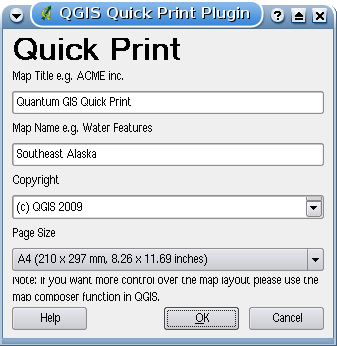
\includegraphics[clip=true, width=6cm]{quick_print_dialog}
\end{center}
\end{figure}

Figura~\ref{fig:quickprint_result} qui sotto mostra il risultato di una stampa veloce DIN A4 dal dataset campione dell'Alaska. Se si vuole maggior controllo sul layout della mappa, è meglio usare il plugin Compositore di Stampe, descritto nella Sezione~\ref{label_printcomposer}.

\begin{figure}[ht]
   \begin{center}
   \caption{Risultato ottenuto con Quick Print come DIN A4 PDF\nixcaption}\label{fig:quickprint_result}\smallskip
   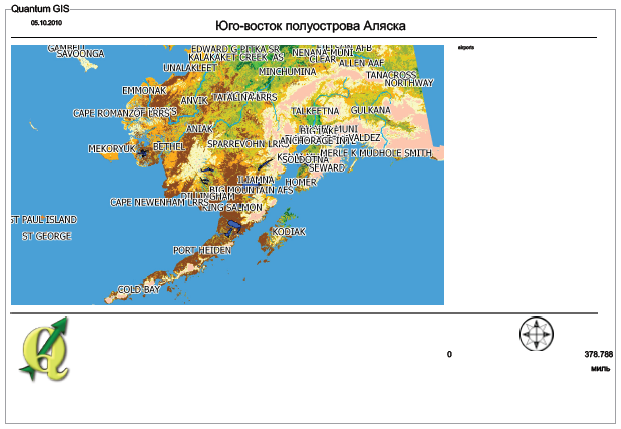
\includegraphics[clip=true, width=11cm]{quick_print_result}
\end{center}
\end{figure}


